%\documentstyle[epsf,twocolumn]{jarticle}       %LaTeX2.09仕様
%\documentclass[twocolumn]{jarticle}     %pLaTeX2e仕様
\documentclass{jarticle}     %pLaTeX2e仕様

%一枚組だったら[twocolumn]関係のとこ消す

\setlength{\topmargin}{-45pt}
%\setlength{\oddsidemargin}{0cm} 
\setlength{\oddsidemargin}{-7.5mm}
%\setlength{\evensidemargin}{0cm} 
\setlength{\textheight}{24.1cm}
%setlength{\textheight}{25cm} 
\setlength{\textwidth}{17.4cm}
%\setlength{\textwidth}{172mm} 
\setlength{\columnsep}{11mm}

\kanjiskip=.07zw plus.5pt minus.5pt

\usepackage[dvipdfm]{graphicx}
\usepackage{ccaption}
\usepackage{algorithm}
\usepackage{algorithmic}
\usepackage{subcaption}
\usepackage{enumerate}
\usepackage{comment}
\usepackage{url}
\usepackage{multirow}
\usepackage{diagbox}
\usepackage{amssymb}
\usepackage{mathtools}
\usepackage{wrapfig}
\usepackage{graphicx}
\usepackage{float}
\usepackage{amsmath}
\usepackage{lipsum}


\begin{document}
  \noindent
  \hspace{1em}

  \today Creation班 ゼミ
  \hfill
  \ \  西村昭賢 

  \vspace{2mm}
  \hrule
  \begin{center}
  {\Large \bf 進捗報告}
  \end{center}
  \hrule
  \vspace{3mm}


\section{2 つのモデルを用いて交互に学習}
2 つモデルを用意し1 つのモデルを対戦相手にして, もう 1 つのモデルを追加で学習できるように実装した.
図 \ref{fig:jikkenimage} に今週行った実験の概略を示す.
\begin{figure}[ht]
  \centering
  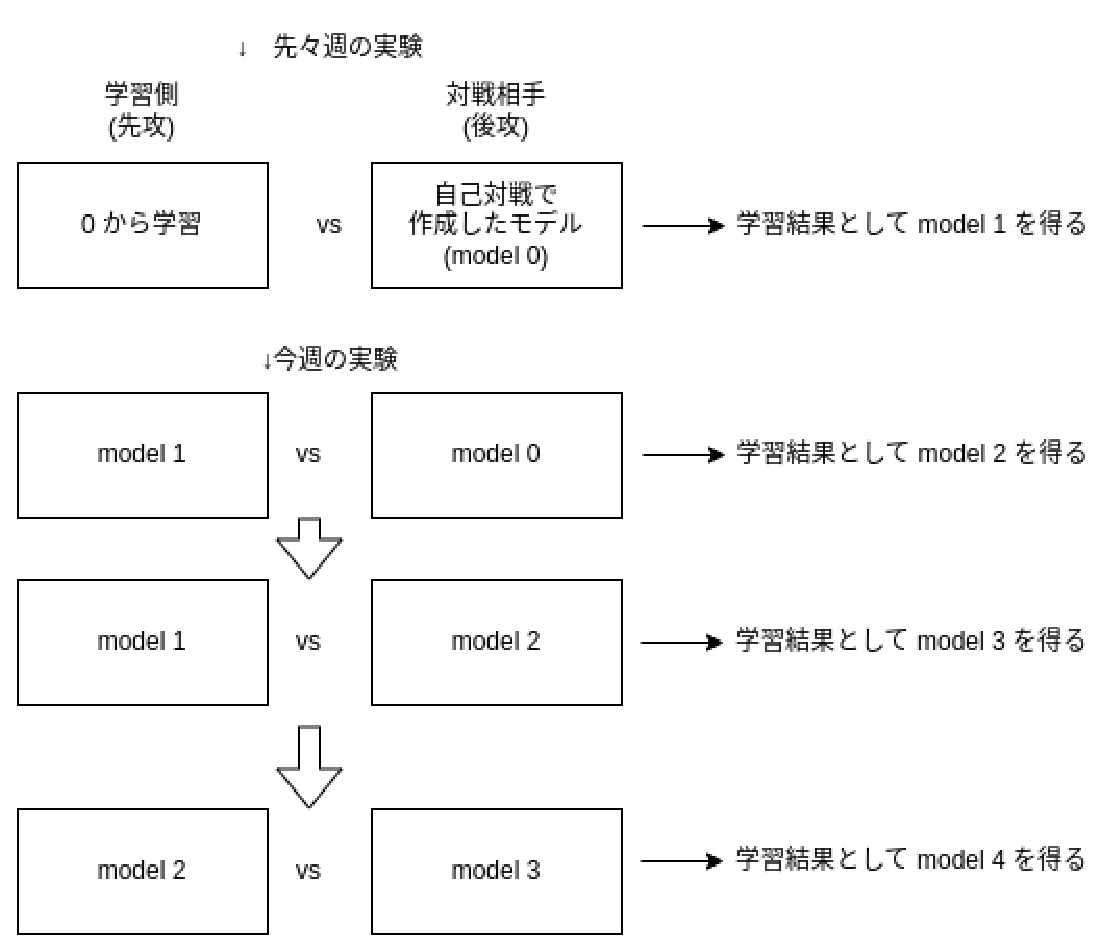
\includegraphics[width=120mm]{assets/jikkenimage.eps}
  \vspace{-0.3cm}
  \caption{今週の実験イメージ図}
  \label{fig:jikkenimage}
\end{figure}

双方ともデッキは同じにして, 1000000ステップ学習させた. 学習後, 10000 回同条件で対戦を行い学習側の勝率を記録した.
図 \ref{fig:model10}, \ref{fig:model21}, \ref{fig:model32} にそれぞれの対戦の学習中の報酬の推移を示している.
\begin{figure}[ht]
  \centering
  \includegraphics[width=120mm]{assets/model1vsmodel0.eps}
  \vspace{-0.3cm}
  \caption{model 1 vs model 0 の報酬の推移}
  \label{fig:model10}
\end{figure}

\begin{figure}[ht]
  \centering
  \includegraphics[width=120mm]{assets/model2vsmodel1.eps}
  \vspace{-0.3cm}
  \caption{model 2 vs model 1 の報酬の推移}
  \label{fig:model21}
\end{figure}

\begin{figure}[ht]
  \centering
  \includegraphics[width=120mm]{assets/model3vsmodel2.eps}
  \vspace{-0.3cm}
  \caption{model 3 vs model 2 の報酬の推移}
  \label{fig:model32}
\end{figure}

特に model 2 vs model 1, model 3 vs model 2 の学習の場合, 学習後の検証段階における勝率はそれぞれ 0.6702, 0.6709 となり, 着実にモデルは強くなっていっていることが考えられる.
また, 図 \ref{fig:model21}, \ref{fig:model32} を見る限り学習済みモデルの重みの読み込みが上手く行えておらず 0 からの学習と等しい推移の仕方をしていると考えられる. 実装を見直してみる.

\section{ChatGPT によるカードプール作成}

ChatGPT にカードプールを作成してもらう実験をした. 前回, 与えたプロンプトが雑なものだったためカードゲームの内容を詳しくプロンプトに記述した. 実際に画面見せて説明します.

\section{今後の課題}
\begin{itemize}
  \item 自己対戦の実装
  \par
  自己対戦の部分の実装で詰まり散らかしてるのでなんとかする. 上手く実装ができなさそうな時は逆転オセロニアの研究で用いられていた HandyRL\footnote[1]{https://github.com/DeNA/HandyRL} など新しいライブラリの導入を試してみたい. 他の強化学習アルゴリズムの検討もありかもしれない.

  \item GA を用いたデッキ構築の実装
  \par
  カードプールから GA を用いてデッキを構築するまでの流れを実装する. 
\end{itemize}



%index.bibはtexファイルと同階層に置く
%ちゃんと\citeしないと表示されない(1敗)
\bibliography{index.bib}
\bibliographystyle{junsrt}

\end{document}